\documentclass[11pt,spanish]{article}

%----------------------------------------------------------------------------------------
% Codificación, y usar una fuente similar a la Palatino (y no Latin Modern Roman)
\usepackage[utf8]{inputenc} % Acentos, etc.
\usepackage[spanish]{babel} % Castellano
\usepackage{tgpagella}      % Fuente similar a Palatino
\usepackage[T1]{fontenc}

%----------------------------------------------------------------------------------------
% TODO
\usepackage{color}
\newcommand{\TODO}[1]{\textcolor{red}{\textbf{\MakeUppercase{#1}}}}

%----------------------------------------------------------------------------------------
% Enumerate with dash instead of period
\usepackage{enumitem}

\makeatletter
\def\twodigits#1{\expandafter\@twodigits\csname c@#1\endcsname}
\def\@twodigits#1{%
  \ifnum#1<10 0\fi
  \number#1}
\makeatother
\AddEnumerateCounter{\twodigits}{\@twodigits}{100}

%----------------------------------------------------------------------------------------
% Indentar primera línea párrafos
\usepackage{indentfirst}

%----------------------------------------------------------------------------------------
% Tablas
\usepackage{eurosym}
\usepackage{multirow}

%----------------------------------------------------------------------------------------
% MODIFICAR EL ESTILO DE LAS SECCIONES 
\usepackage{titlesec}
\titleformat{\section}{\bfseries\Large}{\thesection}{0.8em}{}
\titleformat{\subsection}{\bfseries\large}{\thesubsection}{0.8em}{}
\titleformat{\subsubsection}{\bfseries\large}{\thesubsubsection}{0.8em}{}
\newcommand{\sectionbreak}{\clearpage} % Empezar secciones en nueva página


%----------------------------------------------------------------------------------------
% MODIFICAR EL ESTILO DEL ABSTRACT
\addto{\captionsspanish}{\renewcommand{\abstractname}{\bfseries\large{Resumen}}}
\renewenvironment{abstract}
 {\small
  \begin{center}
  \bfseries \abstractname\vspace{-.5em}\vspace{0pt}
  \end{center}
  \list{}{%
    \setlength{\leftmargin}{7.5mm}% <---------- Cambiar márgenes
    \setlength{\rightmargin}{\leftmargin}%
  }%
  \item\relax}
 {\endlist}
 
%----------------------------------------------------------------------------------------
% Footnotes without line
\makeatletter
\newcommand\footnoteref[1]{\protected@xdef\@thefnmark{\ref{#1}}\@footnotemark}
\makeatother

%----------------------------------------------------------------------------------------
% Imagenes: Que se pongan donde yo quiero
\usepackage{graphicx}
%\usepackage{float}
\usepackage[linecolor=colComment,linewidth=0.65pt]{mdframed}

\usepackage{floatpag} % Pagina en blanco cuando aparece figuras.

\DeclareGraphicsExtensions{.svg,.eps,.ps,.pdf,.png,.jpg,.jpeg}
\addto{\captionsspanish}{\renewcommand{\listfigurename}{\bfseries\Large Figuras}}

%----------------------------------------------------------------------------------------
% Curriculum Vitae
\usepackage{currvita} 
\setlength{\cvlabelwidth}{40mm}

%----------------------------------------------------------------------------------------
% Cronograma: Diagrama de Gantt
\usepackage{gantt}
% Cronograma girado 90º
\usepackage{rotating}
\usepackage{fixltx2e} % poder poner "1ª" en modo texto (no matemático)

%----------------------------------------------------------------------------------------
% COLORES
\usepackage{xcolor}

% Paleta 1
\definecolor{fucsia_cronograma}{RGB}{105,45,172}
\definecolor{naranja_cronograma}{RGB}{255,153,0}
\definecolor{verde_cronograma}{RGB}{87,190,133}
\definecolor{rojo_cronograma}{RGB}{216,117,117}
\definecolor{azul_cronograma}{RGB}{51, 102, 153}
\definecolor{gris_cronograma}{RGB}{143,145,148}
%----------------------------------------------------------------------------------------
% Comenzar con numeracion romana (I,II,III,IV,...)
\renewcommand{\thepage}{\roman{page}}

%----------------------------------------------------------------------------------------
% Definir el titulo

\newcommand{\nombreDelProyecto}{$\mu Search$}

% Comando para multiples saltos de linea
\newcommand{\singlelinebreak}{\\[\baselineskip]}
\newcommand{\multiplelinebreak}[1]{\\[#1\baselineskip]}
\newlength{\drop}

\newcommand*{\titulo}{\begingroup
\thispagestyle{empty}
\drop = 0.13\textheight
\centering
\vfill
\vspace*{\drop}

\includegraphics[scale=0.25]{img/bitparty_big}\singlelinebreak
{\Huge\bf BITPARTY}\multiplelinebreak{2}
{\huge Proyecto \nombreDelProyecto}\multiplelinebreak{2}
{\Large Versión  1.0}\multiplelinebreak{1}
{\Large 03/2014}
\vfill
\vspace*{\drop}
\endgroup}


%----------------------------------------------------------------------------------------
% METADATOS DEL PDF Y PDF CLICKEABLE
\usepackage{hyperref}
\usepackage{hyperxmp}

\hypersetup{
	pdfauthor={Alberto Berbel Aznar, 
				Javier Briz Alastrué, 
				Héctor Francia Molinero, 
				Daniel García Páez,
				Alejandro Gracia Mateo,
				Simón Ortego Parra},
	pdftitle={E20 - Guía de usuario},
	pdfsubject={Proyecto Software. Grado Ing. Informática. EINA. Unizar},
	pdfkeywords={},
	pdfcopyright={Copyright (C) 2014 by Alberto Berbel Aznar, 
				Javier Briz Alastrué, 
				Héctor Francia Molinero, 
				Daniel García Páez,
				Alejandro Gracia Mateo,
				Simón Ortego Parra. All rights reserved.},
	pdfproducer={PDFLatex},
	pdfcreator={ps2pdf},
	colorlinks=false
}

\usepackage[capitalise]{cleveref} % load after hyperref package
\crefdefaultlabelformat{\textbf{#2#1#3}} % boldface only the number

\crefname{figure}{figura}{figuras}
\Crefname{figure}{Figura}{Figuras}

\crefname{listing}{algoritmo}{algoritmos}
\Crefname{listing}{Algoritmo}{Algoritmos}

\crefname{section}{sección}{secciones}
\Crefname{section}{Sección}{Secciones}

%----------------------------------------------------------------------------------------
% FANCY HEADER
\usepackage[head=34pt]{geometry}

\usepackage{fancyhdr}
\pagestyle{fancy}
\fancyhf{} % borrar todos los ajustes

% Configurar la cabecera: fancyhead, fancyfoot para el pie.
\fancyhead[L]{\nouppercase\leftmark}
\fancyhead[R]{\nouppercase\rightmark\hspace{0.5em}}
\fancyfoot[C]{-- \thepage\ --}

% Cabecera parte derecha: número y título de sección, subsección, etc.
\renewcommand{\sectionmark}[1]{\markright{\small{{\bf \thesection} - #1}}}
\renewcommand{\subsectionmark}[1]{\markright{\small{{\bf \thesubsection} - #1}}}
\renewcommand{\subsubsectionmark}[1]{\markright{\small{{\bf \thesubsubsection} - #1}}}

% Cabecera parte izquierda: Nombre de la empresa (logo) y nombre del proyecto
\lhead{\raisebox{-0.5\height}{\rule[-.5ex]{0pt}{2ex}
\includegraphics[scale=0.125]{img/bitparty_small}}\hspace{1em}{\large\nombreDelProyecto}}

\renewcommand{\headrulewidth}{0.6pt} % Tam. separador cabecera
\renewcommand{\footrulewidth}{0pt}   % Tam. separador pie
\renewcommand{\headwidth}{6in}       % Anchura cabecera (incluido separador)

%----------------------------------------------------------------------------------------
%----------------------------------------------------------------------------------------
% INICIO DEL DOCUMENTO
%----------------------------------------------------------------------------------------


%----------------------------------------------------------------------------------------
% PORTADA: TÍTULO
%----------------------------------------------------------------------------------------
\begin{document}
\titulo
\clearpage


%----------------------------------------------------------------------------------------
% ABSTRACT: RESUMEN EJECUTIVO
%----------------------------------------------------------------------------------------
%\thispagestyle{empty}
%\null\vspace{\fill}

%\begin{abstract}
%\paragraph{} Se presenta en este documento la propuesta de proyecto  para el desarrollo de una aplicación web para la venta de microcontroladores a través de un catálogo electrónico, tal y como nos pedía el cliente.
\paragraph{} La aplicación web permite al cliente la búsqueda de microcontroladores en un catálogo electrónico existente, mostrando como resultado un listado sin paginación. 
\paragraph{} El cliente puede añadir desde dicho listado a su carrito de compra los microcontroladores que desee y modificar posteriormente las unidades finales en el carrito de compra, para así poder pedir finalmente la generación de un presupuesto en formato PDF. Cabe recalcar que cada vez que un cliente desee generar un pedido debe introducir sus datos personales y de empresa, es decir, no hay persistencia de los datos.
\paragraph{} Se proporciona además una interfaz web exclusiva para los administradores, a la que solo se accederá desde la empresa cliente de manera local, que tendrán permiso para añadir nuevos microcontroladores al catálogo y modificar y/o eliminar los ya existentes.
\paragraph{} La aplicación entregada a la empresa cliente incluye el servidor web y de base de datos en completo funcionamiento, siendo esto una gran aliciente para la adquisición del producto, pues evita un gasto importante a la empresa cliente. 
\paragraph{} El diseño arquitectural de la aplicación está basado en el patrón Modelo-Vista-Controlador, en concreto, la variante Modelo-Vista-Presentador, separando así de manera notable la vista de la aplicación de los datos de la aplicación, escondiendo así al usuario todos los detalles internos para mayor seguridad de la aplicación.
\paragraph{} En cuanto a detalles tecnológicos de la implementación, concretar que la interfaz web estará implementada con HTML5, CSS3 integrado con el control implementado en PHP5 utilizando el framework CodeIgniter2.1.4 y que se comunica con una base de datos en MySQL5.5. Se asegura además que la aplicación funcionará correctamente en varios de los navegadores web más actuales (Chrome, Mozilla, Opera…).
\paragraph{} Ya presentados los detalles de funcionamiento e implementación de la aplicación, se presentan en el punto final del documento:
\begin{itemize}
\item La división de tareas del proyecto junto a un datagrama, proveyendo así al cliente de una idea bastante exacta de los cumplimientos de plazos previstos.
\item Una oferta económica del desarrollo total de la aplicación.
\end{itemize}
%\end{abstract}


%\vspace{\fill}
\newpage


%----------------------------------------------------------------------------------------
% ÍNDICE
%----------------------------------------------------------------------------------------	
\tableofcontents
\clearpage


% Continuar con numeracion romana (1,2,3...) 
\renewcommand{\thepage}{\arabic{page}}

%----------------------------------------------------------------------------------------
% 2. GUÍA PARA EL USUARIO O CLIENTE HABITUAL
% 2.1 PÁGINA PRINCIPAL
% 2.2 LISTADO COMPLETO DE MICROCONTROLADORES
% 2.3 CARRITO DE COMPRA
% 2.4 GENERACIÓN DE PEDIDO
%----------------------------------------------------------------------------------------
\section{Guía para el usuario/cliente habitual}
\paragraph{}Se presenta aquí la guía para el usuario o cliente habitual del catálogo electrónico de microcontroladores web $\mu$Search. Dicho usuario básicamente utilizará la aplicación para generar un pedido o presupuesto de la compra de varios microcontroladores; navegando por el mismo a través de las funcionalidades típicas de un catálogo electrónico: listado de elementos, búsquedas, carrito de la compra...

\paragraph{}Así pues, a través de los siguientes apartados se guía al usuario a través del proceso que ha de seguir para un uso correcto y eficiente de la aplicación web $\mu$Search consiguiendo finalmente su objetivo, generar un pedido o presupuesto correcto.

\subsection{Página principal}
\paragraph{}Esta es la página principal o de inicio de la aplicación web $\mu$Search. A esta página de inicio, el usuario o cliente habitual será siempre redirigido cuando pulse en cualquiera de los dos logotipos de la cabecera de la página.

\paragraph{}Se le muestra al usuario un mensaje de bienvenida y una breve descripción de en que consiste la página web $\mu$Search, de la empresa creadora y de que se ofrece a través del catálogo electronico.

\begin{center}
	\paragraph{}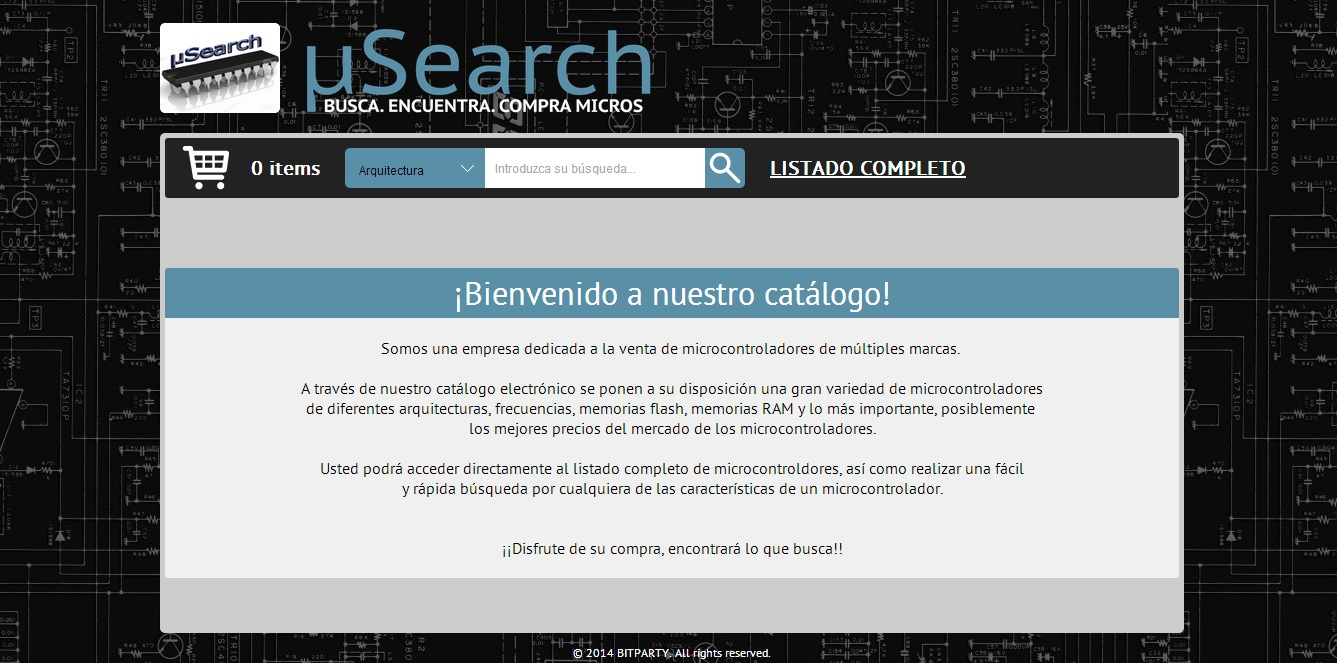
\includegraphics[scale=0.35]{img/principal_user}\singlelinebreak
\end{center}

Desde esta página, a través de los iconos situados en la cabecera debajo de los logotipos de la web, el usuario puede acceder a:
\begin{itemize}
	\item\textbf{Carrito de la compra:} Pulsando sobre este botón el usuario será redirigido a la página del carrito de la compra.
	
	\item \textbf{Búsqueda:} Desde esta sección de la cabecera, el usuario puede realizar búsquedas sobre el catálogo de microcontroladores en base a cualquiera de las diferentes características de un microcontrolador (Arquitectura, Frecuencia, Flash, RAM). Simplemente se debe seleccionar una de las características de la lista despegable, introducir el texto a buscar y pulsar sobre el icono de búsqueda.
	El usuario será redirigido a una página donde se le mostrará el resultado de la búsqueda en forma de lista de microcontroladores.
	
	\item \textbf{Listado Completo:} Pulsando sobre este botón/icono el sistema redirige al usuario a la página en la que se listan todos los elementos disponibles en el catálogo de microcontroladores.
	
\end{itemize}

\subsection{Listado completo de microcontroladores}
\paragraph{}En esta página se puede observar el listado completo de todos los microcontroladores existentes en el catálogo electronico y además, el usuario podrá añadir los que desee al carro de la compra. El listado se muestra en forma de tabla, un microcontrolador por fila, proporcionando información de su nombre, arquitectura, frecuencia, memoria flash, memoria RAM y precio. En la parte derecha de la especificación de cada microcontrolador, se halla el botón de \textbf{\textit{''Añadir''}}, el cual añadirá el producto al carro de la compra actualizando además dinámicamente el número de ítems en el icono del carro incrementándolo en uno.

\paragraph{}Como en todas las demás páginas del sitio web, si se pulsa en cualquiera de los dos logotipos del catálogo $\mu$Search (esquina superior izquierda), el sistema redirigirá al usuario a la página inicial del catálogo.

\paragraph{}Desde esta página, a través de los iconos situados en la cabecera debajo de los logotipos de la web, el usuario puede acceder a:

\begin{itemize}
	\item \underline{\textbf{Carrito de la compra:}} Pulsando sobre este botón el usuario será redirigido a la página del carrito de la compra, donde podrá ver todos los microcontroladores del catálogo electrónico que ha deciddo añadir a su presupuesto, visualizando además el precio total del mismo y pudiendo modificar la cantidad de unidades de los mismos.
	Al lado de este icono, aparece también el número de artículos que han sido introducidos en el carrito; número que se actualiza dinámicamente cada vez que el usuario añada un microcontrolador.
	
	\item \underline{\textbf{Búsqueda:}} Desde esta sección de la cabecera, el usuario puede realizar búsquedas sobre el catálogo de microcontroladores en base a cualquiera de las diferentes características de un microcontrolador (Arquitectura, Frecuencia, Flash, RAM). Simplemente se debe seleccionar una de las características de la lista despegable, introducir el texto a buscar y pulsar sobre el icono de búsqueda.
	El usuario será redirigido a una página donde se le mostrará el resultado de la búsqueda en forma de lista de microcontroladores.
		
	\item \underline{\textbf{Listado Completo:}}Pulsando sobre este botón/icono se recargará la página actual.
\end{itemize}

\subsection{Carrito de compra}
Como en todas las demás páginas del sitio web, si se pulsa en cualquiera de los dos logotipos del catálogo uSearch,
el sistema redirigirá a la página inicial del catálogo.

Debajo de los dos logotipos anteriormente citados se encuentran dos iconos:

\begin{itemize}
	\item[Carrito de la compra] A su lado, aparece también el número de artículos 
	que han sido introducidos en el mismo, pulsando sobre este icono se vuelve a cargar la página actual. Volver a 				
  cargar la página actual puede ser útil en el caso de que se haya modificado la cantidad de uno o varios artículos 			
  del	carrito y se quiera deshacer estos cambios sin que tengan ningún efecto en el precio final de la compra.

	\item[LISTADO COMPLETO] Pulsando sobre este icono el sistema vuelve a la página en la que se listan todos los
	elementos disponibles en el catálogo de microcontroladores.
\end{itemize}

A continuación, se encuentra el listado de los microcontroladores que el usuario ha ido añadiendo al carrito de la 
compra. Este listado, esta compuesto por cuatro columnas: 
\begin{itemize}
	\item[Cantidad] La cantidad de cada elemento añadido al carrito de la compra es un campo modificable que permite
	solicitar más o menos unidades de ese elemento. Para que estos cambios tengan efecto es necesario actualizar el 
	listado como se explica en el apartado siguiente (botón Actualizar).
	
	\item[Referencia] Es el código del fabricante que identifica a cada elemento del catálogo, cada microcontrolador
	tiene una referencia única distinta de las de los demás.
	
	\item[Precio] Es el precio que tiene una unidad.

	\item[Subtotal] Es el resultado de multiplicar el número de unidades solicitadas de un elemento por el precio que
	tiene cada unidad. Hay tantos subtotales como elementos en el carrito de la compra.
\end{itemize}

Debajo del listado de los elementos del carrito de la compra, se encuentran dos botones que pueden tener efecto sobre
todos los microcontroladores solicitados:
\begin{itemize}
	\item[Actualizar] Este botón hay que pulsarlo después de modificar una o varias cantidades de los elementos del 
	carrito de la compra. Es el que permite que dichos cambios tengan efecto. Se puede observar cómo cambia el precio
	Total de la compra. Además, si alguna nueva cantidad tiene un valor de 0, el elemento que tenga dicha cantidad 			
  será eliminado del carrito de la compra.
	
	\item[Vaciar] Pulsando sobre este botón se vacía completamente el carrito de la compra.
\end{itemize}

Antes de finalizar el pedido, hay disponible un formulario que el cliente debe rellenar con sus datos de contacto 
para poder generar correctamente la factura asociada al pedido que se quiere realizar. Todos los campos son obligatorios.

Finamente, una vez que el cliente ha revisado que todos los datos relativos al pedido (cantidades, referencias, precios, 
datos personales, etc.) son correctos hay que pulsar sobre el botón Realizar Pedido para que el sistema genere la 
factura asociada a dicho pedido.

\subsection{Generación de pedido}
Como en todas las demás páginas del sitio web, si se pulsa en cualquiera de los dos logotipos
del catálogo uSearch, el sistema redirigirá a la página inicial del catálogo.

Tras haber solicitado Realizar Pedido, se muestra toda la información relativa al pedido
que se acaba de realizar. Un pedido está compuesto por:

\begin{itemize}
	\item[Tabla de artículos solicitados] En esta tabla se refleja el número de unidades de 
	cada artículo, las referencias, el precio por unidad de cada uno, el precio subtotal para
	cada referencia y el precio final del pedido.
	
	\item[Datos del cliente] Listado con los datos introducidos por el cliente que permiten 
	tanto identificar al cliente como contactar con él si fuese necesario.
\end{itemize}


%----------------------------------------------------------------------------------------
% 3. GUÍA PARA EL ADMINISTRADOR
% 3.1 PÁGINA PRINCIPAL
% 3.2 LISTADO COMPLETO DE MICROCONTROLADORES
% 3.3 AÑADIR MICROCONTROLADOR
% 3.4 EDITAR MICROCONTROLADOR
%----------------------------------------------------------------------------------------
\newpage
\section{Guía para el administrador}
\paragraph{}Se presenta aquí la guía para el administrador del catálogo electrónico de microcontroladores $\mu$Search. El administrador tiene diferentes funcionalidades a las del usuario común, resaltando las de añadir, editar y eliminar microcontroladores de la base de datos.

\paragraph{}Así pues, a través de los siguientes apartados se guía al administrador a través del proceso que ha de seguir para un uso correcto y eficiente de la aplicación web $\mu$Search.

\paragraph{}\underline{\textbf{NOTA:}} Todas las páginas del catálogo electrónico a través de las que navegará el usuario contienen en su parte superior izquierda tanto el logo como el título de la página. Siempre \textit{clickando} sobre cualquiera de los dos el usuario será redirigido a la página principal de administración del catálogo electrónico.

\subsection{Página principal}
\paragraph{}Esta es la página principal o de inicio de la aplicación web $\mu$Search para el administrador de la misma. A esta página de inicio, el administrador será siempre redirigido cuando pulse en cualquiera de los dos logotipos de la cabecera de la página.

\paragraph{}Se le muestra al administrador un mensaje de bienvenida y una breve descripción las funcionalidades que tiene disponibles como administrador de la aplicación web.

\begin{center}
	\paragraph{}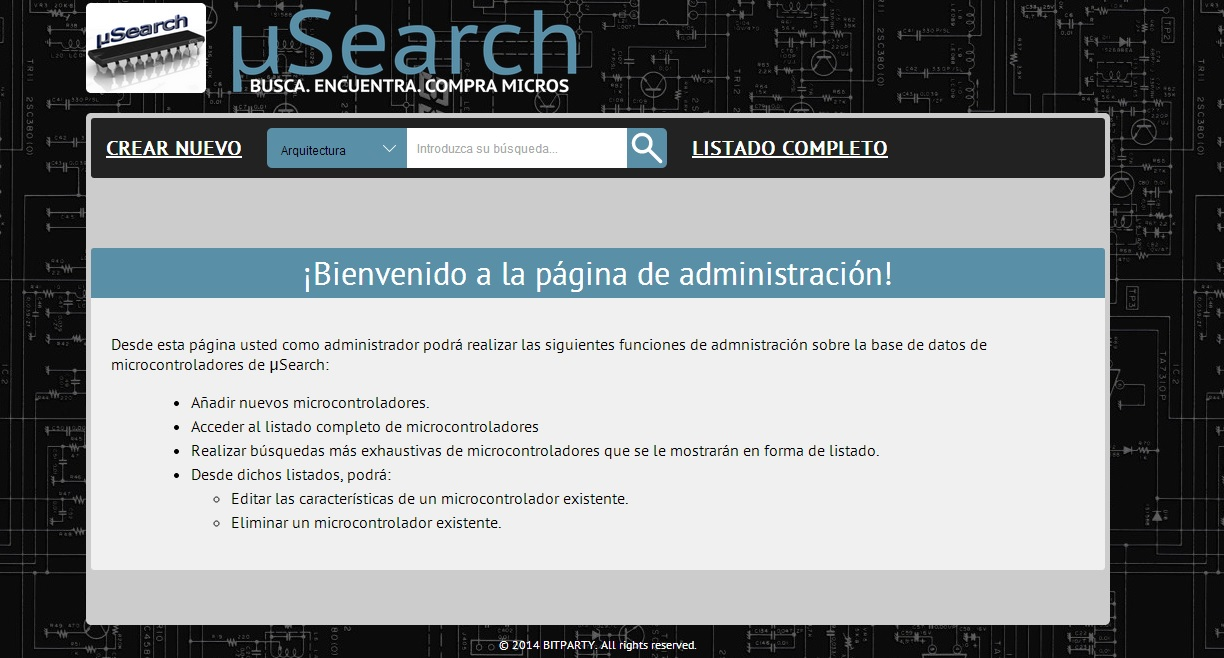
\includegraphics[scale=0.35]{img/principal_admin}\singlelinebreak
\end{center}

Desde esta página, a través de los iconos situados en la cabecera debajo de los logotipos de la web, el administrador puede acceder a:
\begin{itemize}
	
	\item \textbf{Crear Nuevo:} Pulsando sobre este botón el administrador es redirigido a la página que le permitirá añadir un nuevo microcontrolador a la base de datos del catálogo electrónico.
	
	\item \textbf{Búsqueda:} Desde esta sección, el administrador puede realizar búsquedas sobre el catálogo de microcontroladores en base a cualquiera de las características de un microcontrolador (Arquitectura, Frecuencia, Flash, RAM). Simplemente se debe seleccionar una de las características de la lista despegable, introducir el texto a buscar y pulsar sobre el icono de búsqueda.
	El administrador será redirigido a una página donde se le mostrará el resultado de la búsqueda en forma de lista de microcontroladores.
	
	\item \textbf{Listado Completo:} Pulsando sobre este botón/icono el sistema redirige al administrador a la página en la que se listan todos los elementos disponibles en el catálogo de microcontroladores, con sus correspondientes características.
	
\end{itemize}

\subsection{Listado completo de microcontroladores}
\paragraph{}En esta página se puede observar el listado completo de todos los microcontroladores existentes en el catálogo electronico. El listado se muestra en forma de tabla, un microcontrolador por fila, proporcionando información de su nombre, arquitectura, frecuencia, memoria flash, memoria RAM y precio. En la parte derecha de la especificación de cada microcontrolador, se hallan los siguientes botones:
\begin{itemize}
	\item \textbf{Editar:} Redirige al administrador a la página para editar la especificación y características de dicho microcontrolador.
	\item \textbf{Eliminar:} Elimina el microcontrolador de la base de datos del catálogo electrónico, recargando la página con el nuevo listado actualizado.
\end{itemize}

\paragraph{}Como en todas las demás páginas del sitio web, si se pulsa en cualquiera de los dos logotipos del catálogo $\mu$Search (esquina superior izquierda), el sistema redirigirá al administrador a la página inicial de administración del catálogo.

\paragraph{}Desde esta página, a través de los iconos situados en la cabecera debajo de los logotipos de la web, el administrador puede acceder a:

\begin{itemize}
	\item \textbf{Editar:}
	
	\item \textbf{Crear Nuevo:} Lleva al administrador a la página de inserción de artículos, donde se puede rellenar los parámetros necesarios para agregar un nuevo microcontrolador al catálogo electrónico.

	\item \textbf{Búsqueda:} Desde esta sección de la cabecera, el administrador puede realizar búsquedas sobre el catálogo de microcontroladores en base a cualquiera de las diferentes características de un microcontrolador (Arquitectura, Frecuencia, Flash, RAM). Simplemente se debe seleccionar una de las características de la lista despegable, introducir el texto a buscar y pulsar sobre el icono de búsqueda.
	El administrador será redirigido a una página donde se le mostrará el resultado de la búsqueda en forma de lista de microcontroladores.
			
	\item \textbf{Listado Completo:} Pulsando sobre este botón/icono se recargará la página actual.
\end{itemize}

\subsection{Añadir microcontrolador}
\paragraph{} Esta es la página del administrador para añadir nuevos elementos en la base de datos de una manera sencilla. En ella aparecen se le presenta al administrador un formulario con los diferentes campos a rellenar de los microcontroladores que son, uno por caracterísitca:
\begin{itemize}
\item \textbf{Referencia}
\item \textbf{Arquitectura}
\item \textbf{Frecuencia}(MHz) 
\item \textbf{Flash}(Kb)
\item \textbf{RAM(Kb)} 
\item \textbf{Precio($\euro$)}
\end{itemize}

\paragraph{} Al rellenar todos los campos y pulsar el botón \textbf{\textit{''Insertar''}} se añade el elemento a la base de datos y automáticamente se redirigirá al administrador a la página de listado completo, con el nuevo microcontrolador ya incluido en la lista.

\paragraph{}Como en todas las demás páginas del sitio web, si se pulsa en cualquiera de los dos logotipos del catálogo $\mu$Search (esquina superior izquierda), el sistema redirigirá al administrador a la página inicial de administración del catálogo.

\paragraph{}Además, desde esta página, a través de los iconos situados en la cabecera debajo de los logotipos de la web, el administrador puede acceder a:

\begin{itemize}
	\item \textbf{Editar:}
	
	\item \textbf{Crear Nuevo:} Recarga la página actual de creación de un nuevo microcontrolador. El formulario actual no se guarda al recargar la página.

	\item \textbf{Búsqueda:} Desde esta sección de la cabecera, el administrador puede realizar búsquedas sobre el catálogo de microcontroladores en base a cualquiera de las diferentes características de un microcontrolador (Arquitectura, Frecuencia, Flash, RAM). Simplemente se debe seleccionar una de las características de la lista despegable, introducir el texto a buscar y pulsar sobre el icono de búsqueda.
	El administrador será redirigido a una página donde se le mostrará el resultado de la búsqueda en forma de lista de microcontroladores.
			
	\item \textbf{Listado Completo:} Pulsando sobre este botón/icono el sistema redirige al administrador a la página en la que se listan todos los elementos disponibles en el catálogo de microcontroladores, con sus correspondientes características, y desde donde podrán editar o eliminar.
\end{itemize}

\subsection{Editar microcontrolador}
\input{tex/03_4_editar_micro

\end{document}
